%     1.3.1. Ingeniería de proteínas
%         1.3.1.1. Ingeniería de proteínas modulares (a.k.a. quiméricas) (Qué es, 1 página)
%         1.3.1.2. Ejemplos (1 página y 1 figura)
%     1.3.2. Ingeniería de linkers.
%         1.3.2.1. Diseño positivo (propiedades deseadas, 1 página, 1 figura)
%             1.3.2.1.1. Propiedades conformacionales
%             1.3.2.1.2. Carga
%         1.3.2.2. Diseño negativo (propiedades no deseadas, 2 páginas y 1 figura)
%             1.3.2.1.1. Propiedades conformacionales
%             1.3.2.1.2. Propiedades espectroscópicas
%             1.3.2.1.3. Actividades biológicas
%             1.3.2.1.4. Carga metabólica
%         1.3.2.3. Linkers naturales
%             1.3.2.3.1 Características (1 página y 1 figura)
%             1.3.2.3.2 Uso en ingeniería de proteínas (ventajas y desventajas, 1 página)
%         1.3.2.4. Diseño racional
%             1.3.2.4.1 Diseños y conceptos comunes (1 página y 1 figura)
%             1.3.2.4.2 Algoritmos existentes (cómo funcionan, ventajas y desventajas, 2 páginas y 2 figuras)
%             
       
\section{Ingeniería de proteínas}\label{proteinEngineering}
\subsection{Ingeniería de proteínas modulares}    

Como producto de los avances logrados en las tecnologías asociadas al ADN recombinante, se ha desarrollado una nueva generación de proteínas compuestas por la integración
de diferentes módulos secuenciales.

La idea de armar proteínas a partir de la unión de módulos no es algo nuevo sino que sigue la lógica presentada previamente de que las proteínas naturales son usualmente modulares. 
Es decir, se está simulando el proceso evolutivo natural que desarrolla nuevas proteínas mediante la combinación de dominios preexistentes.

La utilización de la técnica de ADN recombinante para construir nuevas proteínas abre toda una gama de posibilidades que van desde inserción de pequeñas secuencias en extremos de proteína naturales, 
con el fin de poder identificarlas o separarlas, hasta el diseño de construcciones proteicas que buscan obtener proteínas con nuevas funcionalidades o propiedades diferentes.
% construidas mediante la combinación de distintos dominios.
% En los casos más simples el proceso puede ser ...
% En el caso de nuevos diseños, donde se busca combinar módulos para dar nuevas funcionalidades o hacerlas más eficientes, el proceso experimental puede ser mas complejo.

% s primeros ejemplos de construcciones artificiales probablemente sean la inserción de epítopes o tags(pequeñas secuencias?) en los extremos de alguna proteína para poder localizarlas y/o separarlas.
% en solución o en el entorno celular.
% Más adelante se desarrollaron nuevas construcciones combinando unidades estructurales y/o funcionales en una sola molécula. 
% Esta fusión de dos o más dominios abre toda una gama de posibilidades para construir proteínas con nuevas o mejores funcionalidades.
% 

% Las distintas bases de datos permiten obtener, entonces, una gran cantidad de módulos estructurales y funcionales y gran parte del diseño de proteínas quiméricas 
% se basa en utilizar estos conocimientos y anotaciones para crear nuevas proteínas con estructuras/funciones/propiedades combinadas.
En los primeros casos el proceso experimental suele ser bastante directo y basta con fusionar un segmento en el extremo deseado de la proteína. 
En los últimos casos de uso, la implementación del proceso experimental tiende a ser más complejo, requiriendo una aproximación de ingeniería. 
En ésta se pueden distinguire varios aspectos de diseño a considerar, los cuales no siempre son totalmente independientes entre si:
% requiriendo un diseño   o un proceso iterativo.
por un lado está el proceso de diseño de la nueva proteína, por otro lado están los aspectos asociados con la técnica experimental de ADN recombinante y expresión de proteinas heterólogas. 
En el gráfico \ref{esquemaProcesoFusion} se representan los pasos generales que pueden formar parte de este proceso.

\begin{figure}[htbp]
\centering
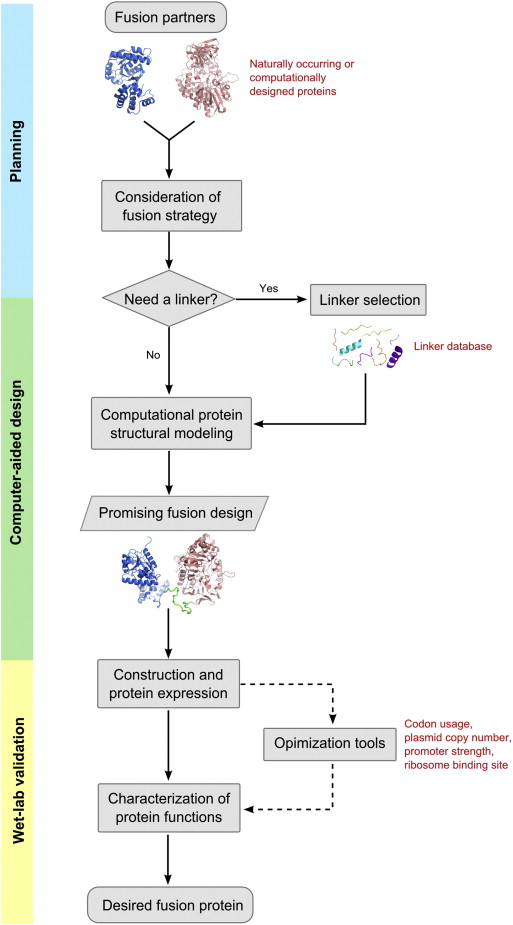
\includegraphics[width=0.7\textwidth]{img/esquemaProcesoFusion.jpg} 
\caption{Figura obtenida de \cite{yu2015synthetic}}
\label{esquemaProcesoFusion}
\end{figure}

El diseño de la proteína de fusión(quimérica) requiere de dos elementos indispensables:
los dominios o proteínas a fusionar, y la secuencia linker que los va a unir.
La elección de los dominios/proteínas está fuertemente ligada al producto final que se desea obtener y, normalmente, es una decisión directa alrededor de la cual se diseña el resto del experimento.
Por otro lado, la selección de un linker adecuado para unir los dominios/proteinas de acuerdo al objetivo que se busca puede ser un paso complicado y es generalmente ignorado cuando se piensa en el diseño de una proteína quimérica.
La unión directa de los dominios/proteínas o el uso de un linker inadecuado puede resultar en resultados indeseables, por ej. puede restringirse la capacidad de plegado de algun dominio globular, 
disminuir el rendimiento de la proteína resultante o la actividad biológica de alguno de los módulos.
La correcta selección, o mejor aún, el diseño racional de las secuencias linker para unir los módulos es un aspecto importante, aunque poco desarrollado, del diseño de proteínas quiméricas. 
Esta falta de desarrollo en el tema se debe quizás a la falta de conocimiento sobre los factores estructurales que gobiernan la flexibilidad entre los dominios, y resulta ser un factor claramente 
limitante en el diseño \textit{de-novo} de proteínas quiméricas. 
Los conocimientos relevantes sobre estos aspectos estructurales de las secuencias linker tema pueden estar disponibles actualmente a partir de la gran cantidad de secuencias que se disponen, los avances en 
la identificación automática de dominios y las nuevas técnicas para predecir propiedades conformacionales a partir de la información secuencial.





% EJEMPLOS

%

% Examples of this approach include green fluores-
% cent protein (GFP) 1 fusion proteins used in cellular localiza-
% tion studies (1), new antibody types such as multivalent
% antibodies and single-chain antibodies (2-7), artificial
% restriction enzymes consisting of zinc-finger and nuclease
% domains (8, 9),


La gran cantidad de posibilidades de aplicación que tiene ingeniería de proteínas quiméricas alienta a seguir investigando 
los aspectos básicos de las proteínas asociados a este proceso y a desarrollar técnicas que ayuden en el prceso de diseño.
Algunos ejemplos de aplicación son: 

% AGREGAR ALGO DE TECNICAS FRET
\begin{itemize}
 \item Creación de enzimas multifuncionales\cite{ljungcrantz1989construction,fan2009engineering}:
% Cómo se dijo en la sección anterior, se poseen cada vez mas dominios anotados con una gran cantidad de funciones correspondientes.
La forma mas común de crear proteinas quiméricas es fusionar genéticamente dos o más dominios con funcionalidades distintas, obteniendo una nueva funcion global para la proteína, resultante de la suma de éstas.
En el caso de enzimas el objetivo generalmente es que una misma construcción pueda tener afinidad por distintos sustratos, o que las distintas enzimas formen una cadena metabólica, donde el producto de una sea a la vez el sustrato de otra.
Es importante que el linker que una a estas distintas enzimas permita la correcta actividad de cada una por separado.

\item Facilitar el estudio de interacciones proteina-proteina\cite{reddy2013linkers}: 
Tradicionamlente, la forma más simple para estudiar la interacción entre dos proteinas es expresarlas conjuntamente para obtener el complejo formado.
Sin embargo, si la afinidad es muy baja, no es tan simple que este complejo se forme de manera estable.
La creación de una proteína quimérica que une a los dominios/proteínas que forman el complejo permite mantenerlas unidas covalentemente mediante una secuencia linker.
La flexibilidad de esta secuencia debería permitir la interacción libre entre los componentes generando la formación del complejo. Al estar unidas covalentemente, habrá una posibilidad mucho mayor de interacción y aumentará la cinética de 
formación, permitiendo realizar los estudios biofísicos necesarios sobre éste.
% The characterization of protein–protein interactions is often required to gain an understanding of various biological processes. 
% Yet, the study of protein–protein interactions for many complexes is hampered when one or more partners of the complex are unfolded or unstable. 
% Traditionally, this problem has been addressed by the co-expression and/or copurification of both proteins. 
% However, for weakly interacting or unstable complexes, the co-expression and/or co-purification often results in a single pro-
% tein. 
% Protein engineering techniques were another
% option to address unfolded or unstable proteins,
% using a single polypeptide chain chimera to link the
% two binding partners via a flexible amino acid linker
% 13
% . With these chimeric proteins, it was then possible
% to maintain both the intramolecular and intermolec-
% ular protein–protein interactions, 14 and chimeric
% proteins have been used to generate stable, soluble
% binary complexes for structural studies, as well as
% functional dimers.
% Linking binding partners using an artificial
% linker will increase the proximity between the inter-
% acting partners and preserve the natural interaction.
% In cases where the interacting partners are not
% linked, it is possible that the binding partners might
% dissociate due to their low affinity and/or due to the
% crystallization conditions.
\item Construcción de sensores FRET:
La técnica FRET se basa en utilizar el efecto de transferencia de energia entre dos cromóforos(un donor y un aceptor).
Dado que la eficiencia en la transferencia, y por lo tanto de la señal de salida, depende de la distancia, este efecto puede ser utilizado en la técnica para evaluar la distancia entre dos 
cromóforos cuya distancia depende de algun proceso molecular de interés. \\
La construcción del sensor generalmente implica utilizar un par de dominios de unión cuya interacción estable depende de algun evento molecular de interés(ej. unión de algún elementos o la ocurrencia de algún proceso).
Cada dominio de unión es unido por separado a uno de los cromóforos(donor o aceptor) y estas construcciones se unen entre si por linkers flexibles que les permiten interaccionar libremente.
En su forma libre, esta construcción permite a los cromóforos moverse de manera independiente por lo tanto no ocurrirá una transferencia significativa de energía. 
Cuando los dominios fusionados a cada cromóforo se unén (lo cual depende de la ocurrencia del evento de interés), la distancia quedará fijada y esto cambiará el perfil de transferencia de energía.
Este esquema se muestra gráficamente en la imagen \ref{fretSensor}

\begin{figure}[htbp]
\centering
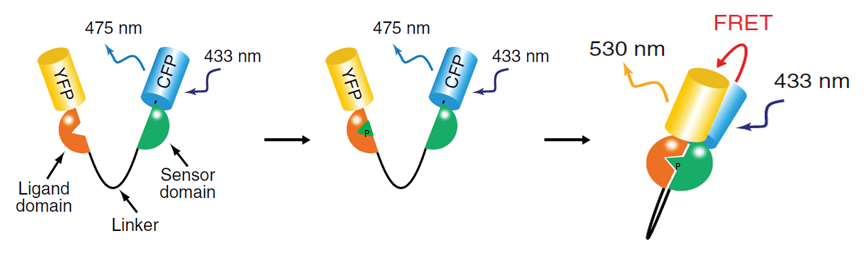
\includegraphics[width=0.7\textwidth]{img/fret.png} 
\caption{Figura obtenida de \cite{crone2013gfp}}
\label{fretSensor}
\end{figure}

Esta técnica es muy versátil y por lo tanto existen una gran cantidad de ejemplos y modificaciones.\cite{vinkenborg2009genetically,qiao2006zinc} %REFERENCIAS
En muchos casos la dependencia del proceso molecular con la distancia esta directamente relacionada con la secuencia linker, 
por ejemplo si esta secuencia contiene elementos target de modificaciones post-traduccionales que pueden cambiar las propiedades conformacionales del linker e, indirectamente, el perfil de distancias entre los extremos. 
En otros casos la conformación en la que los dominios están unidos fija una distancia importante entre los cromóforos, entonces el sensor mide la disminución en la transferencia de energía como evento resultado del evento de interés.
En todos los casos es importante el proceso de ingenieria aplicado sobre el linker para obtener el correcto funcionamiento del sensor.

\item Diseño de métodos de detección para técnicas inmunoquímicas \cite{arai1998construction,arai2000fluorolabeling,suzuki1999open}:
% La unión de fragmentos de anticuerpos a enzimas o proteínas que permitan la detección de la unión es la base de las técnicas inmunoquímicas
Los anticuerpos poseen la capacidad de unirse a proteínas que tengan expuestos epítopes específicos. 
Esta especificidad permite que se usen para identificar la presencia de proteínas de interés en el contexto de diversos métodos experimentales.
% Para poder revelar esta proceso de unión específica es necesario fusionar el anticuerpo con algun elemento que permita la detección, generalmente de forma visual.  
Este proceso, entonces, requiere la utilización de ingeniería de proteínas quiméricas para fusionar el anticuerpo con un dominio cromóforo, una enzima específica, u otro elemento que permita revelar la unión, generalmente de forma visual.


\end{itemize}













\subsection{Ingeniería de secuencias linker}

\subsubsection{Aspectos de diseño}
% EN ESTA  SECCION PONER LA LISTA COMPLETA DE LOS REQUERIMIENTOS POSITIVOS Y NEGATIVOS DE UN LINKER:
% LONGITUD, COMPOSICION, CONFORMACION DESORDENADA INTRINSECA, AUSENCIA DE ESTRUCTURA SECUNDARIA, AUSENCIA DE ELEMENTOS FUNCIONALES

% \subsubsection{Diseño positivo}

La función de la secuencia linker es mantener los dominios unidos a la vez que estos actúan como unidades independientes(manteniendo su funcionalidad), 
permitiendo que se muevan e interaccionen libremente libremente. 
Esta funcionalidad depende directamente de la longitud y conformación adoptada por la secuencia linker, por lo tanto, son los primeros aspectos a tener en cuenta en en diseño.
A pesar de ser un factor directo de la eficiencia\cite{robinson1998optimizing} la longitud no suele ser una propiedad determinante, permitiendo un amplio rango de longitudes efectivas siempre 
que se eviten las secuencias muy cortas que no permiten una separación suficiente, o las secuencias extremadamente largas que haría que los dominios funcionen de forma totalmente independiente entre si.
% harían muy ineficaz la interacción entre proteínas.

Los requerimientos conformacionales suelen ser más estrictos y pequeños cambios en la estructura pueden limitar la funcionalidad del diseño.
En primer lugar buscamos que la secuencia adopte una conformación extendida, es decir, que no se pliege formando una estructura compacta con los dominios que une. 
Además, las propiedades conformacionales de la secuencia deben proveer la flexibilidad necesaria para que las interacciones puedan ocurrir sin ninguna restricción estructural.
Para las arquitecturas más comunes, compuestas de dominios globulares unidos por linkers, esta flexibilidad es el requerimiento mas importante ya que permite a los distintos dominios interaccionar libremente.
Además de esta conformación extendida, es importante controlar 
It is also unfavorable to have a linker sequence with a high propensity for forming alfa-helical or beta-strand structures, because these would limit the flexibility of the fusion protein and consequently affect its functional activity.
Estas propiedades conformacionales tienen una gran correspondencia con las características vistas para las proteínas intrínsecamente desordenadas. 

En la figura \ref{conformacionLinker} se muestran como influyen estos requerimientos en la construcción de una proteína quimérica que une dos dominios EBFP y EGFP. 
Los gráficos A,B y E muestran conformaciones globales de la proteína que son posibles gracias a la flexibilidad del linker intrínsecamente desordenado y con una longitud apropiada. 
Las interacciones que permiten estas conformaciones no se pueden obtener cuando se usa una secuencia con estructura de estructura de hélice-$\alpha$ como se ve en las figuras C y D, donde la rigidez de ésta estructura 
hace que las conformaciones globales sean mucho más limitadas.


\begin{figure}[htbp]
\centering
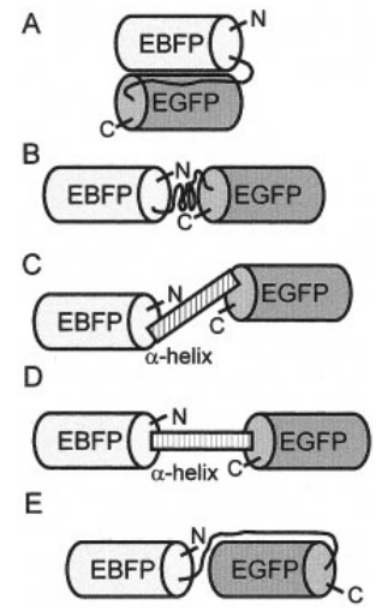
\includegraphics[width=0.3\textwidth]{img/conformacionLinker.png} 
\caption{Figura obtenida de \cite{arai2004conformations}}
\label{conformacionLinker}
\end{figure}



Las características conformacionales buscadas no sólo serán resultado de interacciones intramoleculares sino que dependen del contexto en el cual la proteína diseñada se encuentre. 
Como parte del proceso que describimos en la sección anterior, la construcción se expresa en un sistema biológico determinado, a partir del cual puede ser luego aislada y purificada para estudiar. 
Esto impone ciertos requerimientos al diseño del linker ya que las interacciones estables con otros componentes del sistema pueden limitar seriamente la flexibilidad intrínseca de este.
% MOREs  y Agregacion

Uno de los procesos que pueden afectar más severamente la actividad es la formación de agregados proteicos durante la producción de la proteína\cite{lebendiker2014production}.
En este caso la unión a otras proteínas no solo limita la flexibilidad de la secuencia linker sino también arrastra a la proteína completa inhibiendo completamente la actividad de esta.
Además, la agregación no es sólo un problema de la expresión en el sistema biológico, donde la proteína debe mantenerse en solución,
sino que también puede ocurrir durante las etapas posteriores de separación y purificación.

Otro ejemplo es la uníón a ligandos mediante el proceso de plegado y unión(\textit{binding \& folding}), un proceso mediante el cual se estabilizan estructuras secundarias que de otra modo sólo ocurren en forma transitiva.  
Esta es una propiedad que describimos como característica de las proteínas intrínsecamente desordenadas.
Es importante que el diseño del linker tenga en cuenta estos aspectos(y otros similares), evitando que la secuencia posea tendencias a formar uniones estables con otros componentes del sistema.



% Actividad biologica
Las interacciones desfavorables durante el proceso de ingeniería no se limitan a estas uniones estables.
Como vimos previamente, las proteínas IDPs pueden poseer actividades biológicas, principalmente a través de módulos de interacción en la secuencia. 
Al no adoptar una estructura plegada, estos elementos quedan expuestos al entorno y permiten mediar diferentes interacciones funcionales.
La gama de actividades que involucra a estos módulos es muy diversa y por lo tanto pueden tener diferentes implicancias sobre el linker en particular y la proteína quimérica en general.
% Entre las actividades biológicas asociadas a estos segmentos están las modificaciones post-traduccionales, unión a ligandos, sitios de clivaje, etc.
Ejemplo de esto son los sitios target de clivaje, cuya ocurrencia dentro de la secuencia linker tendría consecuencias obvias que afectarían directamente a la unión covalente que genera el linker.
Otros ejemplos son las modificaciones post-traduccionales sobre la secuencia, las cuales pueden modificar las características de esta(por ejemplo la carga neta) impactando directamente en las propiedades conformacionales asociadas.
% si el linker es target de PTM puede sufrir cambios que afecten la carga de esta secuencia, y como la carga esta directamente relacionada con las propiedades conformacionales, estas modificaciones pueden afectar la flexibilidad
Por lo tanto, es importante que la secuencia linker este libre de cualquier elemento funcional en su secuencia. 

% La idea del diseño uniendo distintos módulos es que la funcionalidad global se origine exclusivamente a partir de la unión de éstos, por lo tanto la secuencia que los une no debe proveer ninguna funcionalidad adicional, es decir,
% debe permanecer inerte ante el entorno en el cual la nueva proteína desarrolla su actividad. 




% COMPOSICION DE AMINOACIDOS: Carga metabolica y propiedades espectroscópicas
Los requerimientos impuestos sobre la secuencia pueden originarse en otros pasos del proceso de producción, no solo en el diseño funcional de la consutrucción 
% por el proceso para producir la proteína quimérica no están limitados a aquellos que apuntan a mantener las propiedades deseadas de la construcción, 
% sino que pueden estar asociados a otros aspectos del proceso.
Como parte de este proceso se requiere que el sistema exprese la construcción diseñada, lo cual, al ser una proteína foránea, estará directamente ligado a la carga
metabólica que la secuencia impone sobre el sistema\cite{glick1995metabolic}. Esta carga metabólica es el resultado de la utilización de recursos propios de la célula para la expresión de esta nueva proteína y dependen, entre otros aspectos, 
de la secuencia que define la proteína. 
Diferentes aminoácidos representan diferentes requerimientos metabólicos, por lo tanto, un aspecto relevante de la secuencia es que esta tenga una composición que imponga mínimos requerimientos metabólicos al sistema. 
La composición raramente puede ser modificada en los módulos que se están fusionando, pero si es posible tener esto en cuenta al diseñar la secuencia linker el cual deberá imponer, idealmente, la mínima carga posible al sistema de expresión.
La importancia de este requerimientos depende del usuario que diseña el experimento, de acuerdo al sistema que se va a usar, el nivel de expresión requerida, etc.

En otros casos, el proceso puede contener requerimientos provenientes de los pasos posteriores a la expresión.
Por ejemplo, dado que las dado que las técnicas espectroscópicas se usan de forma rutinaria en el trabajo con proteínas, es posible que el usuario 
quiera realizar la construcción utilizando un linker cuya composición específica no posea aminoácidos con absorbancia en el rango del UV, 
de forma que se elimine cualquier interferencia de la secuencia en este tipo de técnicas.

Todas estas situaciones están asociadas a requerimientos en la composición del linker diseñado. 
La composición ideal de esta secuencia linker dependerá, entonces, no sólo de las propiedades secuenciales asociadas a la funcionalidad de éste dentro de la construcción, sino también de aquellos aspectos 
que el usuario considere relevantes como parte del proceso experimental.






% 
% 
% 
% % carga neta
% % RESIDUOS CARGADOS
% % Una ventaja importante del proceso de diseño es que se pueda definir la carga neta que tendrá la secuencia linker. 
% % Este requerimiento puede tener varios fundamentos, principalmente 
% Distintas técnicas de laboratorio para identificación y purificación de proteínas se basan en la carga neta de la secuencia.
% 
% 
% Por otro lado, la carga de la secuencia puede mediar interacciones en el entorno celular, por ejemplo, al construir proteínas cuya función requiera unirse al DNA es 
% requerir que la secuencia linker no tenga residos carga ya que 
% 
% Otro ejemplo que afecta a la composición está asociada con interacciones iónicas no deseadas. 
% Por ejemplo al construir una proteína cuya funcionalidad esté asociada a la unión a DNA, será deseable que la composición final no contenga aminoácidos que puedan encontrarse en estados con carga positiva, debido a que 
% la formación de interacciones con la estructura de fosfatos propia del DNA podría interferir en la función de la proteína.
% 
% 
% 
% 




















% % % % % % % ESTO LO PUEDO PASAR A LA PARTE DE LINKERS EMPIRICOS
% 
% % ACA EMPIEZO A HABLAR DE OTROS ASPECTOS NO ESTRUCTURALES
% Sin embargo, la flexibilidad no es todo.  
% Por ej. una opción evidente seria usar linkers de solo Glicina ¿Por qué no usar siempre un linker puramente poli-G, adaptando solamente su longitud?
% Desde los primeros estudios sobre linkers naturales \cite{argos1990investigation} se encontró que las proteinas naturales no usan(seleccionan) este tipo de secuencias.
% Si bien esto no es concluyente para que no se usen, puede darnos un motivo para pensarlo dos veces.
% En primer lugar, un péptido poli-G sería extremadamente inestable y por lo tanto podría actuar como una carga energética, estructural o interferir en procesos de catálisis de los dominios que une, 
% especialmente si tiene una longitud excesiva.
% Se conoce además que el patrón Gly-Gly-X, donde X es un residuo con cadena lateral hidrofóbica, es un sitio target de actividad proteolítica. 
% Por otro lado, una secuencia nucleotídica con alto contenido de Guanina(el codón que codifica para Glicina contiene Guanina en 2 de las 3 posiciones) puede ser difícil de manejar experimentalmente y de expresar para el huésped.
% Como se ve, entonces, existe una gran variedad de aspectos a considerar que exigen distintos requerimientos además de las propiedades conformacionales.
% Por ejemplo, es importante que los linkers should be invulnerable to host proteases, as they are often the targets for degradation. 
% 
% 
% El linker poli-G es sólo un ejemplo. 
% Como vimos en secciones anteriores, distintos elementos funcionales(que actuan principalmente mediante mecanismos de reconocimiento) pueden encontrarse en regiones con distintas propiedades conformacionales. 
% La existencia de estos elementos debe tenerse en cuenta cuando se esta usando la secuencia linker diseñada, y/o su eliminación debe formar parte de la etapa de diseño del linker.
% La longitud del \textit{loop} creado por el linker puede tener un profundo efecto sobre la actividad del linker en una proteína quimérica\cite{nagi1997inverse}.
% Además del ejemplo simple de resistencia proteolítica, las regiones linker también pueden afectar la estabilidad, solubilidad, formación de complejos.
% linker regions can affect the stability, solubility, oligomeric state, and proteolytic resistance ofthe fused protein
% Como se muestra en \cite{robinson1998optimizing}, en algunos casos se tienen efectos importantes variando la longitud y composición de la secuencia
% En base a esto, es esperable que se tengan requerimientos específicos relacionadas con la longitud y la composición. 
% % The stable linkage between functional domains provides many advantages such as a prolonged plasma half-life (e.g. albumin or Fc-fusions). 
% % However, it also has several potential drawbacks including steric hindrance between functional domains, decreased bioactivity, and altered biodistribution and metabolism of the protein moieties due to the interference between domains 
% % In other systems, however, linker regions can affect the stability, solubility, oligomeric state, and proteolytic resistance of the fused proteins
% % Thus, it is important that the length and amino acid composition of a potential linker is optimized in order to preserve the biological activity of the individual proteins in the fused complex.
% 
% 





% \subsubsection{Diseño negativo}




% Además de los analisis sobre las propiedades físicas asociadas a las arquitecturas modulares, el estudio de la diversidad de linkers
% encontrados en la naturaleza puede proveer información importante para entender los requerimientos
% más importantes en el diseño de estas secuencias.


\subsubsection{Linkers naturales}



% 


% El 'descubrimiento' de las regiones/secuencias linkers esta ligado a las teorias de structura-funcion(desarrolladas en la parte de conformacion) que se dieron durante casi 100 años
% En un principio se comenzo a pensar en una estructura rigida asociada a la proteina, luego se fueron revelendo propiedades dinamicas que le permitian cumplir la funcion. 
% Todo esto esta muy asociado a las tecnicas experimentales que se fueron desarrollando.

Como se dijo antes, la modularidad en proteínas naturales es algo muy común y existen muchisimos ejemplos de proteinas multidominio compuestas de dos o mas dominios funcionales unidas por linkers.
Estas secuencias linker sirven, principalmente para mantener unidos los distintos dominios, pero también proveen muchas otras funciones que forman parte de la actividad biológica de la proteína como 
intervenir en las interacciones cooperativas entre los dominios, contener elementos secuenciales que median interacciones con otras proteínas o ligandos, 

El primer estudio realizado sobre secuencias linkers \cite{argos1990investigation} registra la preferencia intrínseca por las conformaciones desplegadas.   
Sin embargo este estudio está bastante desactualizado y los resultados no son representativos ya que se realizó sobre un total de 51 linkers detectados manualmente a partir de 32 proteínas.
En \cite{george2002analysis} se encuentra un análisis más actual sobre un total de 638 proteínas multidominio,  a partir de las cuales se determinaron las regiones linkers(un total de 1280) y dominos utilizando un método automático.

% encuentran los análisis mas detallados donde se estudian las propiedades generales de secuencias linkers naturales

En \cite{chen2013fusion} se revisan los resultados obtenidos en ambos con respecto a diversas propiedades como son longitud, hidrofobicidad, enriquecimiento de ciertos aminoacidos y estructura secundaria adoptada.


% in general, preferable amino acids were polar uncharged or charged
% residues, which constitute approximately 50\% of naturally encoded amino acids. Both
% studies suggested that Pro, Thr, and Gln were the preferable amino acids for natural linkers.

% The preferred linker amino acids observed in the majority of
% the linker sets are Pro, Arg, Phe, Thr, Glu and Gln, in order
% of decreasing preference

Among them, Pro is a unique amino acid with a cyclic side chain which causes a very
restricted conformation [25]. The lack of amide hydrogen on Pro may prevent the formation
of hydrogen bonds with other amino acids, and therefore reduces the interaction between the
linkers and the protein domains.
As a result, the inclusion of Pro residues might increase the
stiffness and structural independence of the linkers.

Proline is unique among protein residues as
it is a cyclic imino acid with no amide hydrogen to donate in
hydrogen bonding. Therefore, it cannot fit into the regular
structure of either $\alpha$-helix or $\beta$-sheet and is a common ``breaker''
of secondary structure.
Proline will introduce some motion into a
helix, that enables a number of different conformations at that
region

Short proline rich sequences are
stiff, with non-interacting connections. As suggested before,
this is the most likely reason why proline is the preferred
linker constituent, particularly in non-helical linkers. It cannot
hydrogen bond to any surrounding amino acids, avoiding
ordered structure formation and contact with the neighbouring
domains.




% PROPIEDADS ESTRUCTURALES

% ESTRUCTURA SECUNDARIA
% Natural linkers adopt various conformations in secondary structure, such as helical, β-strand, coil/bend and turns, to exert their functions.
% the largest proportion of linker residues, 38.3\%,
% adopt the α-helical secondary structure, 13.6\% are in
% β-strands, 8.4\% are in turns and the rest, 37.6\%, are in coil
% or bend secondary structures.


En general, se encontro que los linkers naturales adoptaban principalmente conformaciones desplegadas y tenían estructuras independientes sin interacciones con los dominios adyacentes.
En términos de estructura, por ejemplo, se encontraron tanto linkers flexibles como relativamente rígidos en muchas proteínas.
A través de una mayor rigidez, ciertos linkers pueden ayudar a reducir interacciones no funcionales entre los dominios que unen. 
Por otro lado, una estructura más flexible, como es usual para conformaciones extendidas, provee una mayor flexibilidad y libertad de movimiento a los dominios.


% En \cite{george2002analysis} se esboza una clasificación de los linkers de acuerdo al análisis de su estructura secundaria.
% Se dividen, así, en dos categorías: helicoidales y no helicoidales.
% Los linkers con estructuras de $\alpha$-hélice pueden tener funciones como, por ejemplo, actuar como espaciadores rígidos impidiendo interacciones no funcionales entre los dominios.
% Aunque no sea exhaustiva, esta clasificación permite ver diferencias en los linkers también a nivel de estructura que adquieren, existiendo linkers que, a través de una mayor rigidez, impiden . 




Todas las propiedades analizadas(longitud, composición, hidrofobicidad y estructura secundaria.) resultaron importantes para alcanzar las funciones deseadas.


% AL FINAL DE TODO PONGO ESTOS EJEMPLOS, DEMOSTRANDO QUE LA FUNCIONALIDAD DE LOS LINKERS NO ESTÁ LIMITADA A PROVEER FLEXIBLIDAD Y QUE PUEDEN CUMPLIR OTRAS FUNCIONES

%EJEMPLOS DE PROPIEDADES CONFORMACIONALES
En terminos de flexibilidad, y por lo tanto de propiedades conformacionales en general, los linkers muestran 

en algunos casos la flexibilidad provista por los linkers naturales se origina a nivel de estructura secundaria, y esta limitada a una región corta que funciona como bisagra.
% EJEMPLO!!!!
En otros casos la flexibilidad es ``completa'' y la región del linker es intrínsecamente desordenada\cite{luo2010flexibility}, 
% EJEMPLO !
encontrándose incluso que la funcionalidad de la proteína se pierde cuando se reemplaza por un linker con \cite{hrycyna1998structural}

Ademas, existen linkers que, a pesar de mantener una conformación extendida en solución, pueden plegarse (o fijar una estructura secundaria transitiva) en presencia de ligandos.
Por ejemplo en el caso de ciertas proteínas que se unen a DNA\cite{laity2000dna}
%ESTE ES UN EJEMPLO DE FUNCIONALIDAD 


En algunos casos, las secuencias linker permiten mediar la propagacion eficiente de los efectos originados por la unión de ligandos o modificaciones post-traduccionales en uno de los dominios que conecta(alosterismo).
Un ejemplo es el caso de la miosina del musculo liso, en la cual un dominio que comprende la funcion motora es activado mediante fosforilacion  de una cadena regulatoria unida a este mediante un linker\cite{ikebe1998hinge}.
% OTRO EJEMPLO
% An example is the intramolecular interaction between the Src homology domains (SH2 and SH3) and the catalytic domains of Src family kinases, which results in repression of catalytic
% activity. Repression by the regulatory domain is nullified upon mutation of Trp260 to Ala within the linker separating the SH2 and kinase domain, which proves that the linker plays a crucial role in the coupling of
% the regulatory domains to the catalytic domain



%  ejemplo de la importancia de la secuencia linker en 
% otro ejemplo de funcionalidad esta en  \cite{tsutsumi2012charged}  ...



% CONCLUSIONES
Por lo tanto, a pesar que la flexibilidad es un aspecto que se sabe esta ligado a las secuencias linker en la naturaleza\cite{wriggers2005control}, 
y que estás regiones son generalmente las que permiten los grandes cambios conformacionales en las estructuras de las proteínas, 
estas no son simplemente secuencias que evolucionan hacia conformaciones totalmente flexibles, ya que esto puede no estar directamente ligado al cumplimiento de la función requerida, o no hacerlo de forma eficiente.

De esta forma, las secuencias linker en la naturaleza son una parte mas de las proteínas y sus propiedades conformacionales no pueden definirse como generales, sino que están 
% De esta forma, las propiedades conformacionales de las regiones linkers naturales están usualmente 
asociadas a restricciones funcionales de la proteína global, buscando balancear la flexibilidad requerida 
para que los dominios puedan explorar el ensamble de conformaciones asociado a su funcionalidad, con la rigidez requerida para que no existan interacciones desfavorables entre estos, 
resultando en perfiles muy variados de flexibilidad.

En cada proteina, la secuencia linker puede tener una estructura y una función que haya sido seleccionada para el mecanismo/localización/función de la proteina como un todo, 
y esta función del linker puede no ser solamente la unión covalente de dos dominios. 

Las propiedades funcionales no solo afectan a la conformación sino que abarcan la longitud, composición y propiedades secuenciales puntuales.





% UTILIZACION DE LINKERS NATURALES PARA 
Dado este contexto, el uso de secuencias linkers naturales en el contexto del diesño de proteínas quiméricas debe realizarse con mucho cuidado.
........

% ACÁ PUEDO PONER QUE LOS LINKERS NATURALES TAMBIEN PUEDEN SERVIR COMO BASE PARA UN PROCESO DE INGENIERIA?? O LO PASO A LA PROX. SECCION???









% Los primeros estudios de analisis (estructura y composicion) de secuencias linkers\cite{argos1990investigation} se comenzaron a hacer a partir del analisis estadistico de secuencias que podian ser clasificadas 
% como linkers a partir de las primeras estructuras de proteinas multidominio almacenadas en bases de datos.
% % Estos estudios estaban sesgados por todo el proceso historico de descubrimiento marcado por 
% Los resultados indicaban que la mayoria adquiría una conformación desplegada(tipo \textit{coil}) sin estructura secundaria. 
% % many studies of linker peptides in various protein families have come to the conclusion that linkers lack regular secondary structure (la mayoria se encontraba en estructuraas tipo coil), 
% % they display varying degrees of flexibility to match their particular biological purpose and are rich in Ala, Pro and charged residues
% Asi surgio la idea que los linkers eran secuencias cortas cuya unica funcion era proveer la conexion covalente, lo que estaba de acuerdo con el concepto de hinge-bending.
% Este concepto indicaba que la flexibilidad de estas regiones cortas dentro de un polipéptido permitía el suficiente movimiento a los dominios estructurales.
% % The concept of hinge-bending, whereby the relative flexibility of these short regions of the polypeptide chain allows significant movement of structural domains, gained widespread acceptance in
% % the 1980s and early 1990s, after evidence for conformational transitions in identical or homologous proteins became known.



% A lo largo de los años los conocimientos sobre la composición y propiedades de estas secuencias ha ido cambiando, 
% a medida que mayor cantidad de estructuras se resolvian y mayor conocimiento se obtenia acerca de los dominios que componen 
% las proteinas. Tambien influyeron otras cosas como tecnicas biofisicas que permiten obtener información del ensamble conformacional en solución,
% o algoritmos para automatizar la identificación de los dominios y las secuencias que actúan como linker en una proteina.
% 

% Although the role of linker sequences is likely to be primarily topological, allowing distant parts of the polypeptide chain to interact with diverse partner sequences that might be far apart or close together, 
% linkers and unstructured tail sequences play quite specific roles in a number of systems.








% A FUTURO
Con el incremento del número de estructuras almacenadas en la PDB que ocurrió en los últimos años, sería posible realizar un estudio actualizado de las propiedades de los linkers naturales.
Además, sería interesante extender el número de propiedades analizadas agregando categorías asociadas a función y estructura de la proteína, e identificando la relación entre estas y las propiedades del linker.
% With the rapid increase of the number of protein structures deposited in the PDB database, an updated study of natural linkers could be conducted. 
% In addition to the properties analyzed in previous studies (e.g., amino acid composition, structure classification), 
% it would be interesting to categorize the multi-domain proteins by their functions and structures, and identify the relationship between them and the linker properties


% 
% 
% Based on From George and
% Heringa’s secondary structure analysis, linkers were grouped into two categories: helical and
% non-helical. The $\alpha$-helix was a rigid and stable structure, with intra-segment hydrogen bonds
% and a closely packed backbone [28]. Some $\alpha$-helical conformations form rapidly during
% folding [28], allowing the correct folding of connecting protein domains without non-native
% interactions with the linker. Linkers in an $\alpha$-helix structure might also serve as rigid spacers
% to effectively separate protein domains, and to reduce their unfavorable interactions.
% Therefore, this conformation was commonly adopted by many natural and empirical linkers
% (to be discussed later). On the other hand, without an inherent rigid structure, the non-helical
% linkers tended to be rich in Pro, which could increase the stiffness of the linker as mentioned
% previously [25]. As a result, non-helical linkers with Pro-rich sequence could exhibit
% relatively rigid structures and serve to reduce inter-domain interference.
% 
% 
% 
% Both flexible and relatively rigid peptide linkers are found in many multidomain proteins. 
% Linkers are thought to control favorable and unfavorable interactions between adjacent domains by means of variable softness
% furnished by their primary sequence. Large-scale structural heterogeneity of multidomain proteins
% and their complexes, facilitated by soft peptide linkers, is now seen as the norm rather than the
% exception. Biophysical discoveries as well as computational algorithms and databases have
% reshaped our understanding of the often spectacular biomolecular dynamics enabled by soft linkers.
% Absence of such motion, as in so-called molecular rulers, also has desirable functional effects in
% protein architecture.







% 
% 
% \subsubsection{Molecular rulers}
% These linkers are more defined by their ability to reliably predict and maintain end-to-end distances between attached domains. 
% Such structurally rigid peptides have been conjugated to molecules to serve a metric function.
% These linkers are rich in Proline. 
% Proline is common to many naturally derived interdomain linkers, and structural studies indicate that proline-rich sequences form relatively rigid extended structures to prevent unfavorable interactions between the domains.
% The probable reason why proline is favored over other residues in linking different domains is the inability of proline to donate hydrogen bonds or participate comfortably in any regular secondary structure conformation. This ensures a relatively rigid separation of the domains, thereby preventing unfavorable contacts between them.
% 
% Although short stretches of hard linker sequences are located between functionally relevant regions of protein structure, mutations within such sequences may have no effect on the function.  
% Such linkers are therefore necessary to keep the other amino acid interactions in register, but the nature of the side chain is often unimportant.
% 
% The observed natural tendency to form rigid linkers might also
% be related to avoiding proteolytic cleavage, as linkers are likely
% targets for protease degradation
% 
% Linker
% sequences vary greatly in length and composition, but
% many are rich in polar, uncharged amino acids (such as
% Ser, Thr, Gln and Asn), in the small residues Ala and Gly,
% and in Pro residues. Many of these residues tend to bias
% the polypeptide chain towards the polyproline-II region
% of the RAMACHANDRAN PLOT 27,28 .This means that such
% linkers, although flexible, have a propensity to be highly
% extended. Compositionally biased linker sequences of
% significant length are found mainly in eukaryotic pro-
% teins 1,29 , but short linker sequences of similar composi-
% tion, known as Q-linkers, are also found in a number of
% bacterial regulatory proteins 30 .
% In the absence of their targets, modular proteins
% often behave as ‘beads on a flexible string’, where the
% function of the linker is, primarily, to enable a relatively
% unhindered spatial search by the attached domains 31 .
% However, binding can induce structure formation in
% linkers, which can have significant functional conse-
% quences. For example, the sequence-specific binding of
% CYS HIS ZINC-FINGER PROTEINS to DNA causes the linker to
% fold, cap and thereby stabilize the preceding helix in the
% protein, and to orientate the next zinc finger correctly
% for binding in the major groove of DNA
% 
% 















\subsubsection{Diseño racional}


Con tantos, y tan distintos, requerimientos positivos y negativos, el problema del diseño de linkers puede llegar a ser un tema complejo.
El problema del diseño racional es, entonces, un proceso complicado.
% The general properties of linkers derived from naturally-occurring multi-domain proteins(que se vieron en la seccion anterior) can be considered as the foundation in linker design. 
Las propiedades generales de los linkers naturales encontrados en proteínas multi-dominio pueden considerarse como un primer paso hacia el proceso de diseño.



% PRIMERO HABLAR DE LINKERS USADOS EMPIRICAMENTE 

% Además de la utilización de linkers naturales, una opción común es reutilizar linkers ya utilizados empíricamente, 
La opciones actuales del diseño de linkers se basan, generalmente,  en reutilizar secuencias ya evaluadas empíricamente, buscando la que más se adapte a nuestros requerimientos. 
Muchas de estas secuencias son linkers naturales y otros han sido modificados especificamente en cada caso por procesos de ingeniria.
% Linker engineering, with the aim to control the distance, orientation, and relative motion of two functional domains, will increase in importance with increasing emphasis on the de novo design of multi-domain proteins.
En \cite{chen2013fusion} se hace un análisis de los linkers empíricos más usados para creación de proteínas quiméricas y que pueden encontrarse en literatura, diseñados mediante aproximaciones muy distintas.
A partir de esta recopilación se intenta hacer una clasificación general que resulta en 3 categorias:
linkers flexibles, linkers rígidos, y linkers que pueden experimentar clivaje \textit{in-vivo}. 
Como se puede ver, esta clasificación esta basada, principalmente, en propiedades estructurales/conformacionales. 
Para obtener secuencias que posean otras propiedades de interés deberán analizarse cada uno de los linkers que se detallan en este trabajo.
Los linkers que se encuentran  en la literatura fueron construidos en base a la intuición y la posterior validación experimental.


En el caso de fusiones que requieren linkers flexibles, la mayoría se construye en en base a la intuición utilizando residuos pequeños(polares o no polares) tales como Gly, Ser y Thr,
siendo el linker más común encontrado en la literatura el compuesto por distinto número de repeticiones del motivo $(G_4S_n)$. %PONER REFERENCIAS AL USO DE ESTE.
También se ha utilizado linkers poliglicina($G_n$), en estos casos la sustitución de algunas posiciones por residuos polares (Ser) busca reducir las interacciones no deseadas entre el linker y los dominios que une de forma
tal que no interfieran en la funcionalidad.
Una aproximación de diseño más avanzada se puede ver en \cite{bird1988single}, donde se utilizan residuos Gly y Ser para proveer flexibilidad pero se agregan Glu y Lys para incrementar la solubilidad.
% COMENTAR EL METODO USADO MAS EN DETALLE


% peptide sequences consisting of flexible and hydrophilic residues (arbitrary repeats of glycine and serine residues) are used because they are assumed to form a random coil and do not interact with (the folding of)
% the protein domains
En la mayoría de estos casos, los péptidos con motivos repetidos de Gly y Ser son usados porque se asume que adoptan una conformacion similar a random coil y no interfieren en el plegado y funcionamiento de los dominios que unen,
la funcionalidad provista por estos se evalúa en cada caso en particular.
En \cite{evers2006quantitative} se hace una evaluación de estos linkers tan usados, en el contexto de la unión de dos proteínas fluorescentes, evaluando cuantitativamente las propiedades conformacionales y el efecto de la longitud del linker 
a partir de la transferencia de energía entre estas.


Estos linkers poseen conformaciones desestructuradas (Gly suele considerarse como capaz de romper la estructura ordenada de las hélices), y esta flexibilidad puede, en algunos casos, impedir que se logre una separación 
suficiente entre los dominios (Evers et al., 2006).

As a result, more rigid linkers including polyproline motifs (
Schuler et al., 2005 ) and an all
a-helical linker A(EAAAK)n A(Arai
et al ., 2001) have been developed.




% LINKERS RIGIDOS
% ref 34 = \cite{arai2001design}
% ref 35 = \cite{arai2004conformations}
% 
% An empirical rigid linker with the sequence of A(EAAAK) n A (n = 2-5) was first designed
% by Arai et al. [34, 35]. The linker displayed α-helical conformation, which was stabilized by
% the Glu − -Lys + salt bridges within segments. To test whether they could effectively separate
% the protein domains, these helical linkers were inserted between enhanced blue fluorescent
% protein (EBFP) and enhanced green fluorescent protein (EGFP), and the fluorescent
% resonance energy transfer (FRET) efficiency between EBFP and EGFP was measured [34].
% The FRET efficiency decreased as the length of helical peptides increased, indicating that
% helical linkers can control the distance between domains by changing repetitions of the
% EAAAK motif. Compared to flexible linkers with the same length, the helical linkers
% induced much less FRET efficiency when inserted into EBFP-EGFP fusion proteins,
% suggesting that helical linkers can separate functional domains more effectively.







% PONER LOS EJEMPLOS QUE USAN UNA COMBINACION DE ESTOS LINKERS RIGIDOS Y FLEXIBLES PARA UN DISEÑO DE FRET:
% el linker totalmente flexible permite todo tipo de interacciones entre los dominios, pero
% en este caso lo que se busca es que en la conformacion normal se evite lo mas que se pueda las interacciones entre dominios, ya que estas generan resonancia energetica no deseada(solo se quiere).
% primero: Antibody Detection by Using a FRET-Based Protein Conformational Switch: 
% aca lo que buscan es un linker suficientemente flexible para permitir la interaccion de las dos partes del sensor en su forma no unida al anticuerpo(teniendo asi una alta tasa de emision),
% pero que a la vez permita un 'efficient bridging'(mantenga cierta distancia) como para que, al unirse ambos extremos al anticuerpo, se pierda la interaccion disminuyendo la tasa de emision.
% primero usan un linker super flexible (17 Gly-SerGly repeat), despues prueban uno que incorpora motivos alfa-helice
% El segundo caso donde se usa este nuevo linker es en: a sensor for quantification of macromolecular crowding in living cells
% El linker que terminan usando en ambos es $A(EAAAK)_6A(GSG)_6A(EAAAK)_6A$








% DESPUES EMPIEZO CON DISEÑO RACIONAL

El diseño racional de linkers, sin embargo, está aún en los principios del desarrollo. 


% Although many examples of various types of linkers have been developed in the past, the rational design of linkers for the construction of fusion proteins is still in its infancy. 

En algunos casos se ha 
Existen pocos ejemplos concretos donde se haya utilizado una aproximación racional para el diseño de linkers \cite{arai2001design,arai2004conformations}.

Los estudios detallados de la composición, estructura y función de linkers naturales son un claro punto de inicio.
Con el rápido incremento de los conocimientos sobre la secuencia y estructuras de proteínas, nuevos estudios podrían aportar conocimientos relevantes en esta dirección.
Sin embargo no hay indicios sobre posibles desarrollos orientados a obtener un método sistemático para el diseño racional.  
% Systematic, strategic scientific endeavors are in demand to greatly advance the science of linker design and application.
% Many technology platforms may be investigated in more depth towards understanding the connection between linker composition and structure, and ultimately tie them to linker function.
% The study of linker composition and structure, and the investigation of linker function should go hand in hand when designing a novel linker.
% With the rapid increase of the number of protein structures deposited in the PDB database, an updated study of natural linkers could be conducted.
% The establishment of more databases and searching programs for linkers would be another fruitful direction. 
% As discussed earlier, only two studies have been performed to analyze the characteristics of the linkers in natural multi-domain proteins.
% ESTO ESTA CASI IGUAL EN LA SECCION ANTERIOR

% The extensive studies on the structures of empirical linkers have provided us with useful information for optimal linker design. 
% Ultimately, more searching algorithms for linker databases could be developed, and provide more linker candidates for protein fusion based on user specifications.










% FINALMENTE EXPLICAR LAS APROXIMACIONES RACIONALES QUE ENCONTRE, QUE CONSISTEN BASICAMENTE EN BUSCAR EN BBDD


Los estudios realizados sobre linkers naturales(mencionados en la sección anterior) abrieron la posibilidad de crear bases de datos conteniendo las secuencias encontradas y sus propiedades asociadas.
Asociados a estas bases de datos, se han desarrollado distintos métodos que permiten extraer  ,  que simula un mecanismo de diseño.
% The extensive studies about linkers in natural multi-domain proteins and recombinant fusion proteins fostered the idea of building databases and coming up with linker (designing??) tools 
% to aid the (rational???) design of linkers based on the desired characteristics of fusion proteins.
% Es decir, actualmente la metodologia esta centrada en crear bases de datos de linkers y hacer consultas sobre esta en base a las propiedades que se buscan.

Los resultados del estudio desarrollado en \cite{george2002analysis} son el primer ejemplo de este tipo de metodologías.
% An example of this type of tools was developed during the analysis of a protein dataset to obtain information about linker sequences 
En este trabajo se estudian diversos aspectos asociados a los linkers y se desarrolla una base de datos asociada a un algoritmo de búsqueda que puede ser utilizado mediante un servidor web\cite{linkerdbIBIVU}.
El algoritmo implementado acepta distintos parámetros de búsqueda tales como longitud del linker, accesibilidad del solvente, estructura secundaria adoptada, similitud secuencial con una secuencia input, etc.
% The search algorithm accepts several query types (eg, PDB code, PDB header, linker length, C-alpha extent, solvent accessibility, secondary structure or sequence). 
El programa devuelve las secuencias linker que contienen los criterios solicitados y, además, provee información del contexto en el que se encuentra el linker, con información del ID en PDB, descripciones de la proteína, etc. 
de forma que el usuario pueda inferir otras propiedades del linker que no pueden ser extraídas automáticamente.
% The program can provide the linkers sequences meeting the searching criteria, and also provide other information such as the PDB code and a brief description of the source protein, 
% linker’s position within the source protein, linker length, solvent accessibility, and secondary structure. 
% Users can search for sequences with desired properties, and obtain candidate sequences from natural multi-domain proteins.

Otro ejemplo de búsqueda sobre bases de datos es \url{http://bioinf.modares.ac.ir/software/linda/}

Un ejemplo más reciente de este tipo de aproximación mediante bases de datos da origen a la herramienta LINKER \cite{crasto2000linker,xue2004linker}.
% A more recent example of this type of tool is a program called LINKER 
Al margen de la falta de creatividad en el nombre de la aplicación, esta posee un método de búsqueda que brinda una gran cantidad de opciones al usuario incluyendo aspectos experimentales como la sensibilidad a la actividad de proteasas.
% which searches its database of linker sequences with user-specified inputs (e.g., linker length, protease sensitive sequences to be avoided), and generates an output of several linker sequences that fit the criteria.
En este caso, el centro del método es base de datos conteniendo secuencias loop extraidas de PDB y que son luego levemente procesadas removiento secuencias idénticas, hairpin loops y secuencias de menos de 4 residuos. 
El programa de búsqueda/diseño construido sobre esta base de datos asume que la conformación de loop adoptada por la estructura cristalizada que se encuentra en la PDB dará una conformación extendida 
si se utiliza esta secuencia como linker en una proteína quimérica
Desafortunadamente, el servidor web asociado a este programa no está más disponible.



Una nueva versión de este tipo de soluciones se realizó este año en \cite{liu2015synlinker}. 
La particularidad de esta nuevo programa es que incorpora en su base de datos, no sólo a secuencias linker naturales sino también algunos linkers empíricos extraídos de la literatura, 
que siguen los principios de diseño/construcción que vimos hasta ahora en esta sección.
Una particularidad de esta herramienta es que permite obtener un modelo computacional donde 1 o mas linkers se fusional con estructuras/dominios obtenidos de la pdb. 
Este modelo puede ser usado directamente como input en el próximo paso(siguiendo el esquema de la figura \ref{esquemaProcesoFusion}) donde se pueden evaluar mediante simulaciones de dinámica molecular algunas propiedades conformacioneles de la construccion obtenida.



A pesar que las bases de datos no proveen una solución total al problema de diseño, la construcción de estas y los métodos de búsqueda asociados 
ayuda a la utilización de los conocimientos adquiridos a partir de estudios sobre secuencias naturales.
% building an empirical linker database could help summarize the knowledge and facilitate the future linker design.
% The extensive studies on the structures of empirical linkers have provided us with useful information for optimal linker design. 
El desarrollo de métodos de búsqueda más abarcativos junto con nuevos estudios para encontrar secuencias linker naturales podría generar un avance en este tipo de metodologías.
% Ultimately, more searching algorithms for linker databases could be developed, and provide more linker candidates for protein fusion based on user specifications.
% Lo bueno de las BBDD es que los elementos que contienen suelen haber sido probados experimentalmente, lo cual es fundamental.








































% In summary, linkers can adopt various structures and exert diverse functions to fulfill the  application of fusion proteins (Table 2). 
% The flexible linkers are often rich in small or hydrophilic amino acids such as Gly or Ser to provide the structural flexibility and have  been applied to connect functional domains that favor interdomain interactions or
% movements. In cases where sufficient separation of protein domains is required, rigid linkers may be preferable. 
% By adopting α-helical structures or incorporating Pro, the rigid linkers can efficiently keep protein moieties at a distance. 
% Both flexible and rigid linkers are stable in vivo, and do not allow the separation of joined proteins. Cleavable linkers, on the other
% hand, permit the release of free functional domain in vivo via reduction or proteolytic cleavage. They can be utilized to improve the bioactivity of chimeric proteins, or to  specifically deliver prodrugs to target sites where the linkers are processed to activate bioactivity. The rational choice of linkers should be based on the properties of the linkers
% and the desired fusion proteins.

% 
% % FLEXIBLE LINKERS
% Flexible linkers are usually applied when the joined domains require a certain degree of movement or interaction. They are generally composed of small, non-polar (e.g. Gly) or polar (e.g. Ser or Thr) amino acids
% Este tipo de polipeptidos do not affect the function of the individual proteins to which they attach. 
% 
% The small size of these amino acids provides flexibility, and allows for mobility of the connecting functional domains. 
% The incorporation of Ser or Thr can maintain the stability of the linker in aqueous solutions by forming hydrogen bonds with the water molecules, and therefore reduces the unfavorable interaction between the linker and the protein moieties.
% The most commonly used flexible linkers have sequences consisting primarily of stretches of Gly and Ser residues (“GS” linker). 
% By adjusting the copy number “n”, the length of this GS linker can be optimized to achieve appropriate separation of the functional domains, or to maintain necessary inter-domain interactions.
% The loop length created by the linker can have a profound effect on the action of the linker in the fused complex
% 
% Many other flexible linkers have been designed for recombinant fusion proteins. As suggested by Argos [23], these flexible linkers are also rich in small or polar amino acids such as Gly and Ser, but can contain additional amino acids such as Thr and Ala to maintain flexibility, as
% well as polar amino acids such as Lys and Glu to improve solubility.
% 
% 
% 
% % LINKERS RIGIDOS (MOLECULAR RULERS)
% While flexible linkers have the advantage to connect the functional domains passively and
% permitting certain degree of movements, the lack of rigidity of these linkers can be a
% limitation. There are several examples in the literature where the use of flexible linkers
% resulted in poor expression yields or loss of biological activity.
% 
% The ineffectiveness of flexible linkers in these
% instances was attributed to an inefficient separation of the protein domains or insufficient
% reduction of their interference with each other. Under these situations, rigid linkers have
% been successfully applied to keep a fixed distance between the domains and to maintain their
% independent functions
% 
% The major concern in the design of a molecular ruler is the possibility of softening and structural failure that arises when the ruler is unable to provide a predictable separation distance between its bound
% moieties. An adequate cushion distance is often required when designing the linkers.
% 
% Alpha helix-forming linkers with the sequence of (EAAAK) n have been applied to the
% construction of many recombinant fusion proteins [18, 20]. As suggested by George and
% Heringa [24], many natural linkers exhibited $\alpha$-helical structures. The $\alpha$-helical structure
% was rigid and stable, with intra-segment hydrogen bonds and a closely packed backbone
% [28]. Therefore, the stiff $\alpha$-helical linkers may act as rigid spacers between protein domains.
% 
% 
% Another type of rigid linkers has a Pro-rich sequence, (XP) n , with X designating any amino
% acid, preferably Ala, Lys, or Glu. As suggested by George and Heringa [24], the presence of
% Pro in non-helical linkers can increase the stiffness, and allows for effective separation of
% the protein domains. The structure of proline-rich sequences was extensively investigated by
% several groups
% 
% Un ejemplo interesante, relacionado con la aplicacion que motivó este trabajo(FRET) se puede ver en (ref Design of the linkers which effectively separate domains of a bifunctional fusion protein - Ryoichi Arai,): 
% En este trabajo.....
% An empirical rigid linker with the sequence of A(EAAAK) n A (n = 2-5) was first designed.
% The linker displayed  $\alpha$-helical conformation, which was stabilized by
% the Glu Lys salt bridges within segments. To test whether they could effectively separate
% the protein domains, these helical linkers were inserted between enhanced blue fluorescent
% protein (EBFP) and enhanced green fluorescent protein (EGFP), and the fluorescent
% resonance energy transfer (FRET) efficiency between EBFP and EGFP was measured [34].
% The FRET efficiency decreased as the length of helical peptides increased, indicating that
% helical linkers can control the distance between domains by changing repetitions of the
% EAAAK motif. Compared to flexible linkers with the same length, the helical linkers
% induced much less FRET efficiency when inserted into EBFP-EGFP fusion proteins,
% suggesting that helical linkers can separate functional domains more effectively.
% 
% 
% % IN-VIVO CLEAVABLE LINKERS
% Under these circumstances, cleavable linkers are introduced to release free functional
% domains in vivo . The design of in vivo cleavable linker in recombinant fusion proteins is
% quite challenging. Unlike the versatility of crosslinking agents available for chemical
% conjugation methods, linkers in recombinant fusion proteins are required to be
% oligopeptides. The linkers introduced in this section take advantage of the unique in vivo
% processes, and are cleaved under specific conditions such as the presence of reducing
% reagents or proteases. This type of linker may reduce steric hindrance, improve bioactivity,
% or achieve independent actions/metabolism of individual domains of recombinant fusion
% proteins after linker cleavage
% 



